\chapter{Literature Review} \label{chap:literatureReview}

%\version{v1.10.2015}

Pet Diet and Health care Planner is important for our daily life which is used by the pet owner. Pets are the member of our family and it is very important to take care of them. The application will help pet owner to take care of their beloved pets and keep in touch with by proper diet plans, treatment suggestions and take appointment or contact with pet doctor in case of emergency. Some other applications that are in market are as follows:
\section{Dog Walk \cite{capsix}}
It is application for both android as well as IOS users. The application is very helpful. The application users can perform multiple tasks through this application; for example user can track and record   pet daily routine base activities like walk of dog. The walk is recorded when pet owner or user turn on the GPS in his mobile. Through this application pet owner can see the moves of his dog but the application is confined to the walk of your dog. Pet diet plans, diseases details and treatment suggestions are missing.
\begin{figure}[H] 
  \centering
    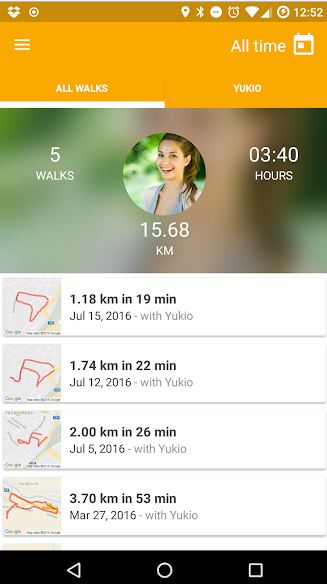
\includegraphics[scale=0.3]{21dogwalk}
     \caption{Dog Walk}
\end{figure}
\section{My Pet Reminders\cite{capseven}}
My pet Reminder is mobile base application for android and IOS mobile user. This is useful in making a pet profile, generating a reminder of pet important dates for example birthday or appointment but the pet diet, diseases, treatment suggestions and healthcare services functionalities are not the part of this application currently.
\begin{figure}[H]
  \centering
    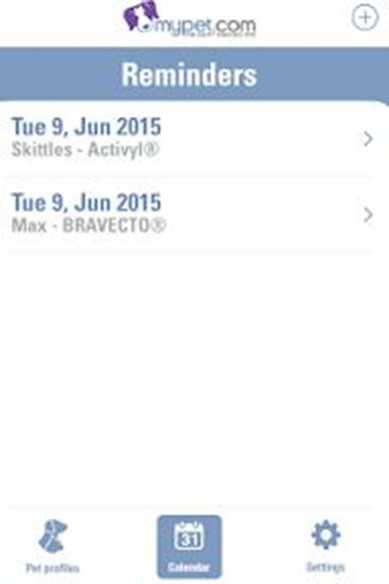
\includegraphics[scale=0.3]{22MyPetRemainder}
     \caption{My Pet Reminders}
\end{figure}
\section{Dog Sync\cite{capseight}}
It is web portal. This is very useful application in recording pet activities for example when the pet watered, when the pet walked, when the medicine is given and when the pet is fed. User can also share this record with the friends and other users of this application. This web application lacks the pet diet plans and diseases details and some other necessary healthcare services. This application is limited to only dogs. Android version and IOS version of this application is currently not available.
\begin{figure}[H]
  \centering
    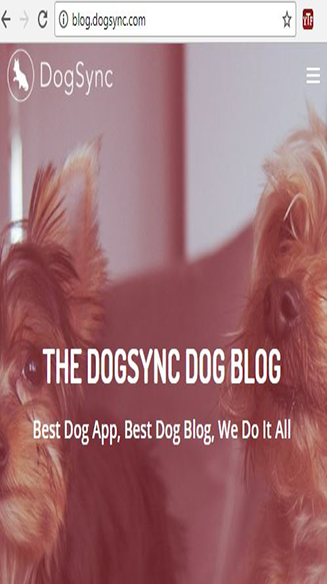
\includegraphics[scale=0.3]{23DogSync}
      \caption{Dog Sync}
\end{figure}
\section{ASPCA Pet Safety\cite{capsnine}}
The ASPCA has multiple applications for the pet owners regarding safety and locating the pet in case the pet is lost. The ASPCA Pet Safety app is available for both Android, IOS users. this application can help pet owners plan for pet safety during emergencies, natural disasters and extreme weather. The app teaches safety and preparedness hints, it also suggestions on how to search for lost pets right after emergencies and tools for storing pet information or creating a lost pet kit. The drawback of using this application is that it does not provide important functionality like, this application does not provide any monitoring of the health of the pet. It does not provide access to a vet for appointment and checkups.
\begin{figure}[H]
  \centering
    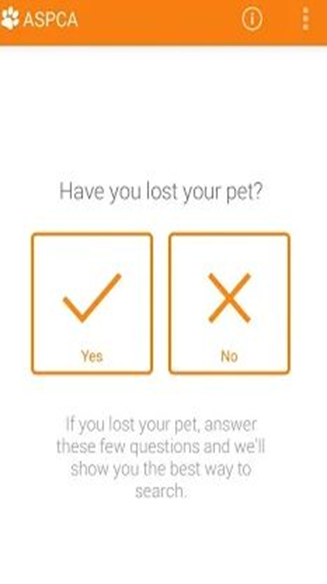
\includegraphics[scale=0.3]{24ASPCAapp}
      \caption{ASPCA Pet Safety}
\end{figure}
\section{Dog Health[9]}
This app is used because it generates  reminders about the appointments with your vet. The drawback of this application is that this application does not keeps track of the previous visits to the vet  and does not store any medication administration that has to be done. Overall this application is very is not useful.The only function that  this application performs is generating alerts.
\begin{figure}[H]
  \centering
    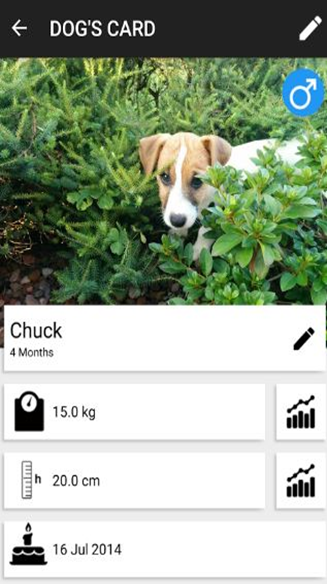
\includegraphics[scale=0.3]{25Doghealth}
     \caption{Dog Health}
\end{figure}
\section{Pet Coach\cite{petcoach}}
Pet coach is a complete platform for the web, android and IOS users. The application generates the advices and tips for pet’s health from the professional pet doctors. After installing this application anyone can post the question related to his pet diet, behavior and training. Consultations are free and well as paid for the users. Although pet coach is a very useful application but this is limited to take an appointment or advises from the doctor. While weekly and daily diet plan, pet common diseases, treatment plan and notifications features are considered as out of scope now.
\begin{figure}[H]
  \centering
    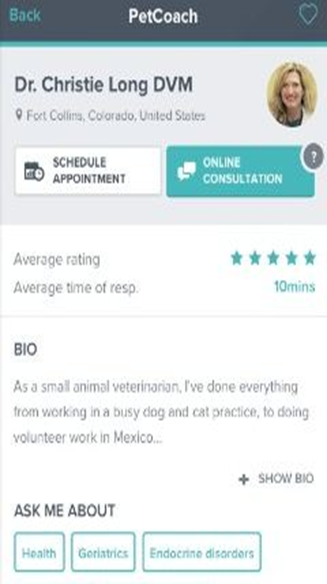
\includegraphics[scale=0.3]{26petcoach}
      \caption{Pet Coach}
\end{figure}
\section{Pet-First Aid\cite{petfirstage}}
Pet-First Aid based upon a very unique idea by American android and IOS developer Red Cross. Application includes the photos, videos, tips and first aid guidelines in case of emergency or injury. If the injury of the pet is very severe then the application can view the hospital list located nearby or contact the pet doctor. While using this application user can’t view the diet plan, common diseases, treatment plan and notification features.
\begin{figure}[H]
  \centering
    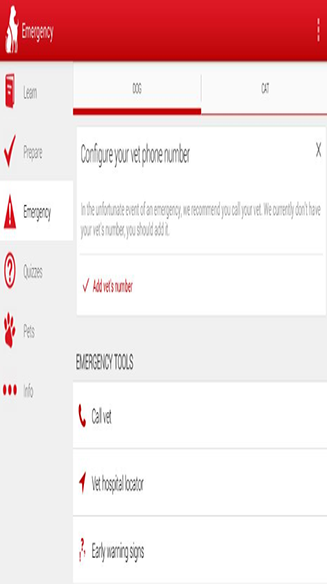
\includegraphics[scale=0.3]{27petfirstaid}
    \caption{Pet-First Aid}
\end{figure}
\section{Rover\cite{capsrover}}
Rover is complete platform web, android and IOS users.  It basically establishes the network of such persons who are dog owner. Dog owners usually find too much difficulty in finding the sitters and boarding. This application is limited to provide facility to the dog owners in booking sitters for their dogs for boarding purpose, finding dogs care center, and send notifications to the pet users related to the updated photos of home sittings. Although this is very useful but confined to the dogs day care centers and homes. 
\begin{figure}[H]
  \centering
    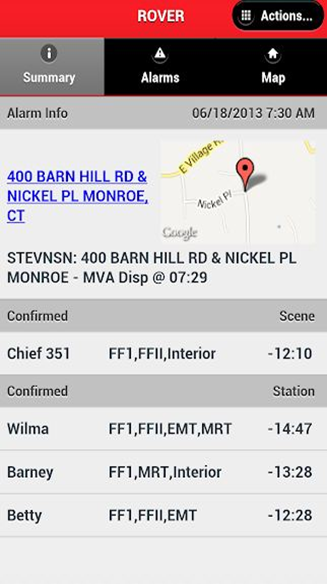
\includegraphics[scale=0.3]{28rover}
      \caption{Rover}
\end{figure}
There are many mobile applications which are related to pets but few are discussed in details. Most of them work on the specific single feature; for example Rover is an application which helps in searching the dog day care centers. Pet First Aid helps in searching out the pet hospitals in case of emergency. Pet Coach helps in taking out the advises and tips from the professional pet doctor. Dog Health is confined to the dog health only. ASPCA Pet Safety helps the pet owners in the case of pet loss. Dog walk is limited to record the walk and activities of dog. My Pet Remainder helps to notify the owner related to important dates of his pet like birthday etc. “Pet Diet and Health care Planner is focusing on many features like generate pet diet plan, diseases details, generate alarm  notification on pet food time and take an appointment.








